% EN49 c05 | 原书 p.48–57（PDF 59–68） | 第 3 章（无小节）
\section{纤维的补集}

% ===== 原书 p.48 =====
本章先记录若干简单观察，主题是 Landau--Ginzburg 模型 $(X\times\C,\,z(f-t))$ 随 $t$ 变化的几何。
本节约定 $f_t(z)=f(z)-t$。

首先注意，$z(f-t)$ 只有一个临界纤维，出现在 $z(f-t)=0$ 处。
该纤维作为集合由 $(f^{-1}(t)\times\C)\cup(X\times\{0\})$ 给出；临界轨迹恰为 $f^{-1}(t)$。
注意当 $t\ne0$ 时，该临界轨迹因而光滑，我们得到显式的局部 Morse--Bott 模型，细节见下。

对 $\eps\ne0$，$z(f-t)$ 在 $\eps$ 上方的光滑纤维为
\[
  \{(x,z): f(x)\ne t,\ z=\eps/f_t\},
\]
作为集合可等同于补集 $X\setminus f^{-1}(t)$。
该补集上相应的 Liouville 结构来自 Stein 函数到纤维的限制。

\transnote{易错预警：临界纤维作为集合是 $(f^{-1}(t)\times\C)\cup(X\times\{0\})$，比临界轨迹 $f^{-1}(t)$ 大一圈。$X\times\{0\}$ 那部分不是临界点，只在集合层面属于奇异纤维，勿把它算进临界轨迹。}

% ===== 原书 p.49 =====
利用因子 $\C$ 上的 Stein 函数 $|z|^{2n}$，这一结构由
\[
  \psi(x)=\phi(x)+\frac{\eps^{2n}}{|f_t(x)|^{2n}}
\]
给出。该 Stein 函数也可这样得到：取 $X\setminus f^{-1}(t)$ 到 $\C^{N+1}$ 的嵌入
$x\mapsto(i(x),\eps/f_t(x))$。

\transnote{易错预警：$\eps$ 是 $\C$ 方向上的取值，不是形变参数。$z=\eps/f_t$ 自带 $1/z$ 型行为，故 $\psi$ 中出现的是 $|f_t|^{-2n}$ 而不是 $|f_t|^{2n}$；指数取反就换成了另一个 Stein 结构。}

我们改用补集上一个形变等价的 Stein 结构，它由
\[
  \psi(x)=\phi(x)+\frac{C\phi(x)}{|f_t(x)|^{2n}}
\]
给出，其中 $C>0$ 与 $n\in\N$ 取合适的值。
该 Stein 函数来自 $X\setminus f^{-1}(t)$ 到 $\C^{2N}$ 的嵌入
$x\mapsto(i(x),\sqrt{C}\,i(x)/f_t(x)^n)$，并与前一结构 Stein 形变等价；形变为
\[
  \psi_s(x)=\phi(x)+\frac{s+\phi(x)}{1+s\phi(x)}\frac{C}{|f_t(x)|^{2n}},
  \qquad s\in[0,1].
\]

\transnote{含糊点拨：两处「Stein 结构」并不相同，但只差一个 Stein 形变。按引理 \ref{lem:simple-homotopy}，形变只改变 Liouville 结构、不改 wrapped Fukaya 范畴的拟等价类，故后面可以随意换用。}

要理解 $t\ne0$ 与 $t=0$ 时 $(X\times\C,z(f-t))$ 的 LG 模型如何不同，需要研究一般纤维的 Liouville 结构如何变化。
下面这个初等例子说明了做法。

\begin{example}\label{exam:3-0-1}
我们回忆如何在 Lefschetz 纤维丛上构造标准 Weinstein 结构。
考虑标准 Lefschetz 纤维丛 $f\colon\C^2\to\C$，并给 $\C^2$ 配标准 Stein 结构。
考察纤维 $f^{-1}(t)$ 的补集的骨架。
当 $t=0$ 时，$\C^2\setminus f^{-1}(0)=(\C^*)^2$ 带标准 Liouville 结构，故其骨架对应于零截面 $T^2\subseteq T^*T^2\cong(\C^*)^2$。

% ===== 原书 p.50 =====
\begin{figure}[htbp]
  \centering
  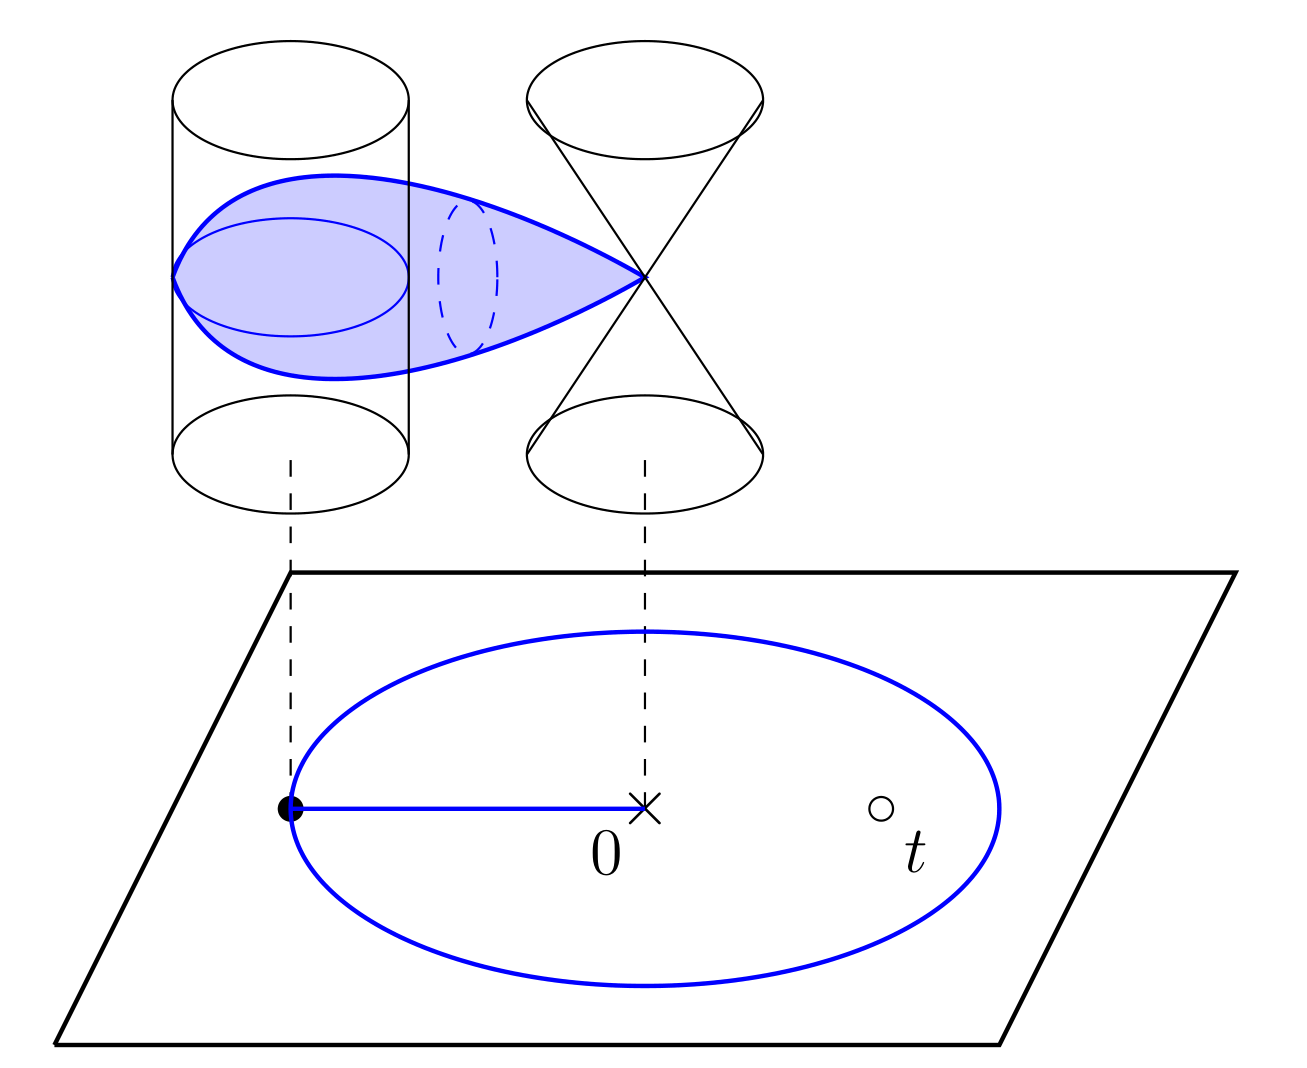
\includegraphics[width=0.42\textwidth]{figures/fig3_1.png}
  \caption{例 \ref{exam:3-0-1} 中的骨架（蓝色）。}
  \label{fig:3-1}
\end{figure}

注意，$\C^2$ 上 Stein 结构给出的 Weinstein 函数在 $0$ 处只有一个临界点，指标为 $2$。
取 $t\ne0$ 后，$X\setminus f^{-1}(t)$ 上的 Weinstein 函数现在包含这个临界点。
因此 $\C^2\setminus f^{-1}(t)$ 由 $\C^2\setminus f^{-1}(0)$ 附加一个临界 Weinstein 把手得到。
$\C^2\setminus f^{-1}(t)$ 的骨架现在包含该把手的核，它附着在原来的 $T^2$ 上，见图 \ref{fig:3-1}。\hfill$\Box$
\end{example}

\transnote{背景直觉：例子说明的是「挖掉的纤维从 $0$ 移到 $t$」这一动作。$t\ne0$ 时 $0$ 处那个临界点落进了补集，于是补集相当于在 $T^2$ 上粘了一个把手；命题 \ref{prop:3-0-3} 把这幅图景推广到一般 $X$。}

为描述一般情形，我们需要引理 \ref{lem:local-psi-outward} 的对偶版本。

\begin{proposition}\label{prop:3-0-2}
  对充分大的 $C>0$、$n\in\N$ 以及充分小的 $t$，$\psi$ 的 Liouville 向量场在 $\{|f_t|^2=\delta\}$ 上内指，
  对一切充分小的 $\delta>0$ 成立。
\end{proposition}

\begin{proof}
考察内积
\[
  \langle\nabla_X|f_t|^2,\nabla_X\psi\rangle
  =\Bigl(1+\frac{C}{|f_t|^{2n}}\Bigr)\langle\nabla_X|f_t|^2,\nabla_X\phi\rangle
  -\frac{nC\phi}{|f_t|^{2n+2}}|\nabla_X|f_t|^2|^2 .
\]

% ===== 原书 p.51 =====
由 Cauchy--Schwarz 不等式，只要
\[
  2\Bigl(\frac{|f_t|^{2n+2}}{C}+|f_t|^2\Bigr)
  <n|\phi|^{1/2}|\nabla_X|f_t|^2|,
\]
在 $|f_t|^{-1}(\delta)$ 上就有 $\langle\nabla_X|f_t|^2,\nabla_X\psi\rangle<0$。
再次取 $|t|,\delta>0$ 充分小，可保证对某个充分大的 $n\in\N$，Malgrange 条件在 $|f_t|^2=\delta$ 上成立，命题得证。
\end{proof}

\transnote{易错预警：命题 \ref{prop:3-0-2} 是引理 \ref{lem:local-psi-outward} 的对偶，结论却是「内指」。差别出在负指数上：$\nabla_X|f_t|^{-2n}$ 带出因子 $-2n|f_t|^{-2n-1}$，故末项为 $-\dfrac{nC\phi}{|f_t|^{2n+2}}|\nabla_X|f_t|^2|^2$，符号与引理 \ref{lem:local-psi-outward} 的正指数项相反。}

\begin{remarkx}\label{rem:8}
注意可以把上述论证中的 $\phi$ 换成与引理 \ref{lem:local-psi-outward} 的 Stein 函数同伦的 Stein 函数
\[
  \psi=\phi+C\phi|f_t|^{2m},
\]
从而让引理 \ref{lem:local-psi-outward} 与命题 \ref{prop:3-0-2} 同时成立（在同心的圆盘上）。所得不等式
\[
  C|f_t|^2+|f_t|^{2n+2}+D|f_t|^{2m+2n+2}
  <\frac{\phi^{1/2}}{2}|\nabla_X|f_t|^2|\bigl(Cn-Dm|f_t|^{2m+2n}\bigr)
\]
在 $\eps\le|f_t|^2\le\delta$ 上成立，其中 $\delta>\eps>0$ 充分小，$C,n$ 在给定 $D,m$ 后取得充分大。
\end{remarkx}

\transnote{含糊点拨：本条不等式给出两套构造同时成立的充分条件，不是新的估计。右端括号 $Cn-Dm|f_t|^{2m+2n}$ 须为正，这就是先取 $C,n$、再取 $D,m$ 的顺序不能颠倒的原因。}

现在我们用 Eliashberg 的 Weinstein 流形手术理论，来理解一般纤维随 $t$ 的变化：

\begin{proposition}\label{prop:3-0-3}
  上述 $X\setminus f^{-1}(t)$ 上的 Weinstein 结构，由 $X\setminus f^{-1}(0)$ 附加一族 Weinstein 把手得到。
\end{proposition}

% ===== 原书 p.52 =====
\begin{proof}
先说明如何从 $X\setminus f^{-1}(0)$ 过渡到 $X\setminus f^{-1}(B_\delta)$，两者都配 Stein 函数
\[
  \psi_0(x)=\phi(x)+\frac{C\phi(x)}{|f(x)|^{2n}}.
\]
由命题 \ref{prop:3-0-2}，对充分小的 $\delta>0$ 与充分大的 $n,C$，可取 $B_\delta$ 为 $0$ 处的球，
使 $\psi_0$ 在 $X$ 上的 Liouville 向量场沿 $|f|^{-1}(\delta)$ 内指。
再把 $\delta>0$ 缩小，可使 $f^{-1}(B_\delta\setminus\{0\})$ 中没有该 Liouville 向量场的零点，
因为 $\phi$ 在 $X$ 上的零点在映射 $f\colon X\to\C$ 下是孤立的。
于是 $X\setminus f^{-1}(0)$ 与 $X\setminus f^{-1}(B_\delta)$ 之间有一个平凡的 Weinstein 配边，
因而有 Liouville 流形的同构 [CE12]。

取 $|t|<\delta$，现在从 $X\setminus f^{-1}(B_\delta)$ 过渡到 $X\setminus f^{-1}(t)$。
首先，$X\setminus f^{-1}(B_\delta(s))$ 上有一族 Weinstein 结构形变（对 $|s|<\delta$ 都微分同胚）：
\[
  \psi_s(x)=\phi(x)+\frac{C\phi(x)}{|f_s(x)|^{2n}},\qquad s\in[0,t].
\]
对充分小的 $\eps>0$，$\psi_s$ 在 $f^{-1}(B_\delta)$ 之外的临界点当 $s$ 从 $0$ 变到 $t$ 时都不进入 $f^{-1}(B_\delta(s))$：
故这是简单 Liouville 形变，于是 $\psi_0$ 与 $\psi_t$ 在 $X\setminus f^{-1}(B_\delta)$ 与 $X\setminus f^{-1}(B_\delta(t))$ 上给出同构的 Liouville 结构（引理 \ref{lem:simple-homotopy}）。

现在，由于 $\psi_t$ 的 Liouville 向量场沿 $f^{-1}(\partial B_\delta)$ 内指，
注意 $f^{-1}(B_\delta)\setminus f^{-1}(t)$ 给出从 $X\setminus f^{-1}(B_\delta)$ 到 $X\setminus f^{-1}(t)$ 的 Weinstein 配边。
于是由 Eliashberg 的 Weinstein 流形手术理论 [CE12]，沿 $X\setminus f^{-1}(B_\delta)$ 的边界附加

% ===== 原书 p.53 =====
\begin{figure}[htbp]
  \centering
  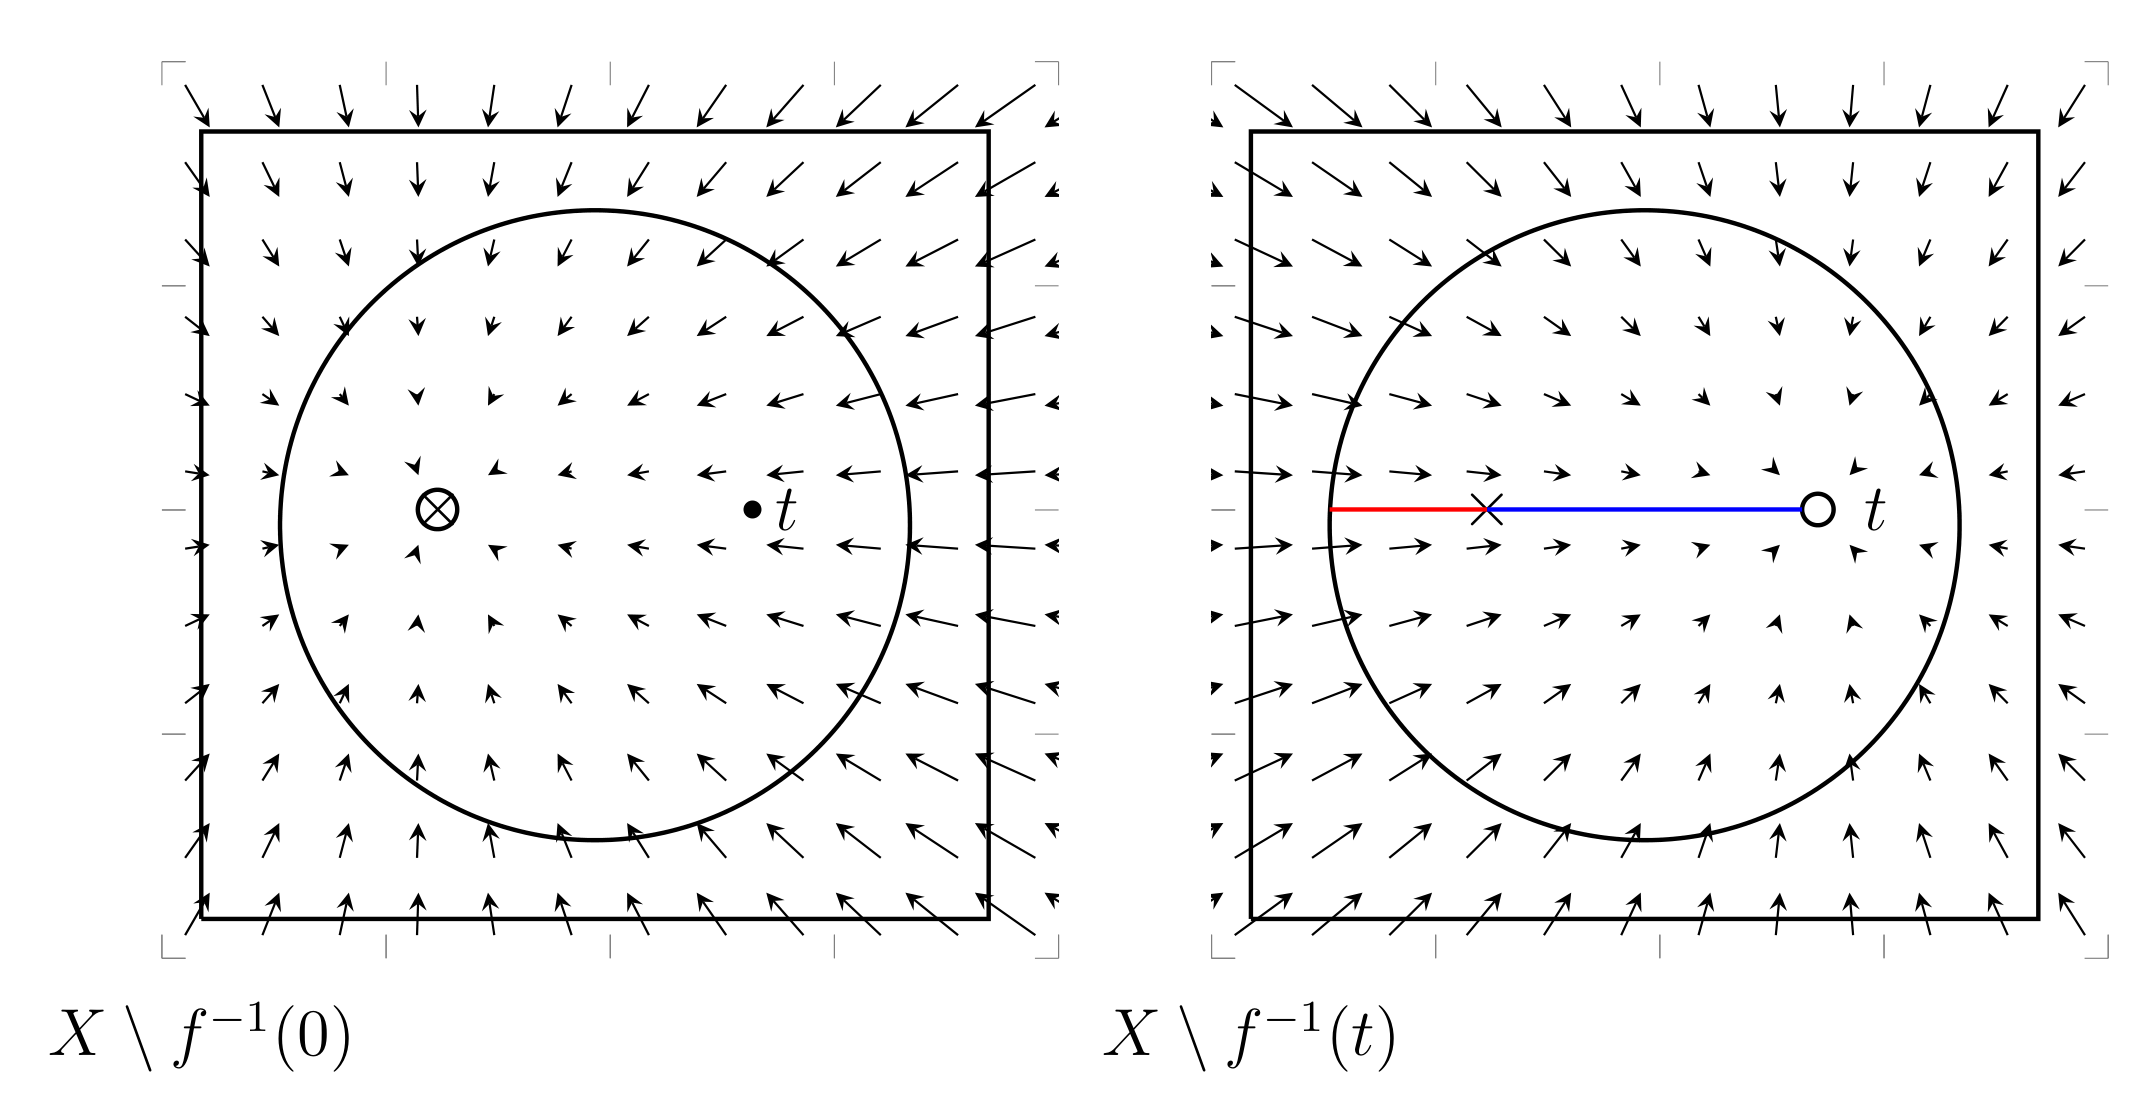
\includegraphics[width=0.86\textwidth]{figures/fig3_2.png}
  \caption{命题 \ref{prop:3-0-3} 的把手附加过程：新增把手的核为红色，余核为蓝色。}
  \label{fig:3-2}
\end{figure}

Weinstein 把手，即得 $X\setminus f^{-1}(t)$：见图 \ref{fig:3-2}。
\end{proof}

命题 \ref{prop:3-0-3} 给出的临界把手统称为\textbf{附加把手}（additional handles）。
应用 Ganatra--Pardon--Shende 的去停点定理 [GPS19, Theorem 1.16]，我们得到：

\begin{proposition}\label{prop:3-0-4}
  取上述构造的 Liouville 结构，则有范畴等价
  \[
    \cW(X\times\C,zf)\cong\cW\bigl(X\times\C,z(f-t)\bigr)/\cD,
  \]
  其中 $\cD$ 是 $\cW(X\times\C,z(f-t))$ 的满子范畴，由 $X\setminus f^{-1}(t)$ 中附加把手的稳定流形的环绕圆盘张成。
\end{proposition}

\transnote{易错预警：命题 \ref{prop:3-0-4} 的商是「满子范畴 $\cD$ 的商」，不是对理想或对对象取商。$\cD$ 由附加把手稳定流形的环绕圆盘张成，与命题 \ref{prop:3-0-5} 的余核是同一批几何对象的两个侧面。}

\begin{proposition}\label{prop:3-0-5}
  对上述 Stein 流形 $X$ 上的函数 $f$，范畴 $\cW(X,f)$ 由附加把手的余核分裂生成。
\end{proposition}

% ===== 原书 p.54 =====
证明中我们会说明附加把手的余核（记作 $\ell_i$）在什么意义下是 $\cW(X,f)$ 的对象。

\begin{proof}
先研究 $X\setminus f^{-1}(B_\delta)$ 的 wrapped Fukaya 范畴，其 Stein 结构为
\[
  \psi(x)=\phi(x)+\frac{C\phi(x)}{|f(x)|^{2n}},
\]
其中 $\delta,C,n$ 如命题 \ref{prop:3-0-3} 的证明中所取。
如注 \ref{rem:8} 那样，通过改变 $\phi$ 可得某个 $R>\delta$，使 $\psi$ 的 Liouville 向量场沿 $|f|^{-1}(R)$ 也外指。
为此我们想如下加入停点：
\begin{itemize}
  \item 停点 $F$，由 $f^{-1}(-R)$ 给出；
  \item $|f|^{-1}(\delta)$ 上的停点 $\Lambda$，由附加把手 $\ell_i$ 所沿附着的带标架 Legendrian 球面 $\Lambda_i$ 给出。
\end{itemize}
由生成性结果 [GPS19, Theorem 1.10]，$\cW(X\setminus f^{-1}(B_\delta),F\cup\Lambda)$ 由两类拉格朗日对象生成：
\begin{itemize}
  \item $F$ 与 $\Lambda_i$ 的环绕圆盘；
  \item 由 $f^{-1}(t)$ 的余核与连接 $-R$ 到 $|f|^{-1}(\delta)$ 的弧 $\gamma$ 的乘积给出的拉格朗日对象 $L$。
\end{itemize}
用 [GPS19, Theorem 1.9] 的缠绕正合三角形，可以把 $F$ 的环绕圆盘用 $L$ 与 $\Lambda_i$ 的环绕圆盘的扭复形表示，如图 \ref{fig:3-3}。
注意取乘积所用的弧 $\gamma$ 在复平面中位于停点 $F,\Lambda$ 之下。

% ===== 原书 p.55 =====
\begin{figure}[htbp]
  \centering
  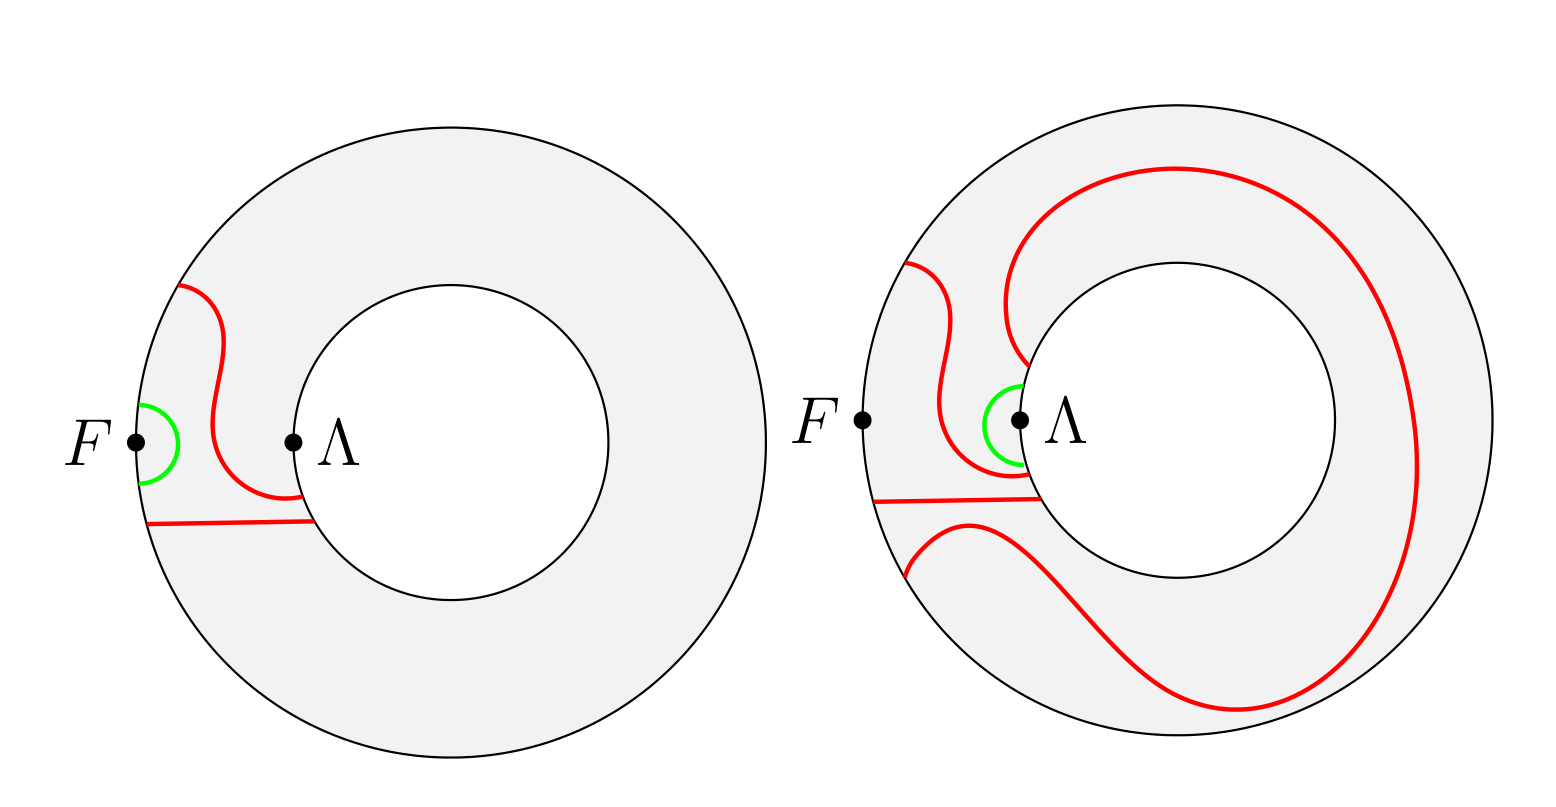
\includegraphics[width=0.78\textwidth]{figures/fig3_3.png}
  \caption{由对象 $L$（红色）与 $\Lambda$ 的环绕圆盘（绿色）造出 $F$ 的环绕圆盘。}
  \label{fig:3-3}
\end{figure}

\transnote{易错预警：图中弧 $\gamma$ 必须画在停点 $F,\Lambda$ 之下。缠绕正合三角形的符号与「上下」约定绑定，画反了会得到相反的同调移位。}

现在依命题 \ref{prop:3-0-3} 附加 Weinstein 把手，过渡到 $(X\setminus f^{-1}(t),f)$，同时保持 Liouville 向量场沿 $|f|^{-1}(R)$ 外指。
此时 $\Lambda_i$ 的环绕圆盘恰好变成附加把手的余核 $\ell_i$，
于是由 [GPS19, Theorem 1.20] 的粘合结果知，$\cW(X\setminus f^{-1}(t),f)$ 由附加余核 $\ell_i$ 与拉格朗日对象 $L$ 生成（参看 [GPS19, p.68]）。
可以把这些 $L$ 取为在从 $-R$ 到 $f^{-1}(t)$ 的弧 $\gamma$ 上纤维化、且经过 $f$ 的奇异纤维之下、停点 $F$ 之下的对象。

现在考虑 Weinstein 形变
\[
  \psi_t(x)=\phi(x)+\frac{C\phi(x)}{|f_t(x)|^{2n}}.
\]
与注 \ref{rem:8} 类似地论证：对一切充分小的 $\eps>0$，可选 $\phi$、更大的 $C,n$ 与更小的 $R,\delta$，
使得存在某个 $R'>R+\eps$，满足 $|f|^2$ 的 Malgrange 条件失效的所有点都落在 $|f|\le R'+\eps$ 之外，并且
\begin{itemize}
  \item 当 $0<|t|<R+\eps$ 时，$\psi_t$ 在 $X\setminus f^{-1}(t)$ 上的 Liouville 向量场沿 $|f|^{-1}(r)$ 外指，其中 $R'+\eps>r\ge R'$；

% ===== 原书 p.56 =====
  \item 当 $R+\eps/2<|t|<R+\eps$ 时，该 Liouville 向量场沿 $|f|^{-1}(R)$ 外指。
\end{itemize}

第一个性质防止 Liouville 域的骨架逃出某个紧集之外，
故 $\psi_t$ 给出 $X\setminus f^{-1}(t)$ 在 $0<|t|<R+\eps$ 时的简单 Weinstein 形变。
于是所得的 $X\setminus f^{-1}(t)$ 彼此正合辛同胚，wrapped Fukaya 范畴 $\cW(X\setminus f^{-1}(t),f)$ 保持不变（引理 \ref{lem:simple-homotopy}）。

$\psi_t$ 在 $R+\eps/2<|t|<R+\eps$ 时的第二个性质意味着：由于停点 $F$ 位于 $|f|^{-1}(-R)$ 之内，
我们得到 $(X\setminus f^{-1}(t),f)$ 的一个子扇形 $(f^{-1}(B_R(0)),f)$；见图 \ref{fig:3-4}。
应用 Viterbo 限制，对象 $L$ 与 $\ell_i$ 分裂生成 $\cW(f^{-1}(B_R(0)),f)$（由 [Syl19c, Theorem 1.8]）。
但 $(f^{-1}(B_R(0)),f)$ 与 \S2 中用于定义 $\cW(X,f)$ 的原始扇形 Weinstein 形变等价，形变为
\[
  \psi_{t,s}(x)=\phi(x)+C\phi(x)\rho_s(f_t(x))
\]
其中 $s\in(0,1]$，$\rho_s(z)=\beta_s(|z|)/|z|^{2n}$，$\beta_s\colon\R\to[0,1]$ 是光滑截断函数，取法满足
\[
  \beta_s(r)=
  \begin{cases}
    1 & \text{当 } r\le\tan(\pi s/2),\\
    0 & \text{当 } r\ge\tan(\pi s/2)+\eps,
  \end{cases}
\]
并使 $\rho_s(f_t(x))$ 多重次调和（这里 $\psi_1=\psi$）。
此外，对一切 $s\in(0,1]$，$\psi_{t,s}$ 的 Liouville 向量场在 $R+\eps>|t|>r\ge R+\eps/2$ 时沿 $|f|^{-1}(r)$ 保持外指，故这实际上给出简单 Weinstein 形变。

\transnote{背景直觉：Viterbo 限制把整体范畴的生成元压到子扇形上，这一步是「先局部生成、再回到整体」的枢纽。子扇形只保留 $|f|\le R$ 的部分，故 $\beta_s$ 必须把 $f_t$ 截断在 $R$ 附近，同时保持多重次调和性。}

% ===== 原书 p.57 =====
\begin{figure}[htbp]
  \centering
  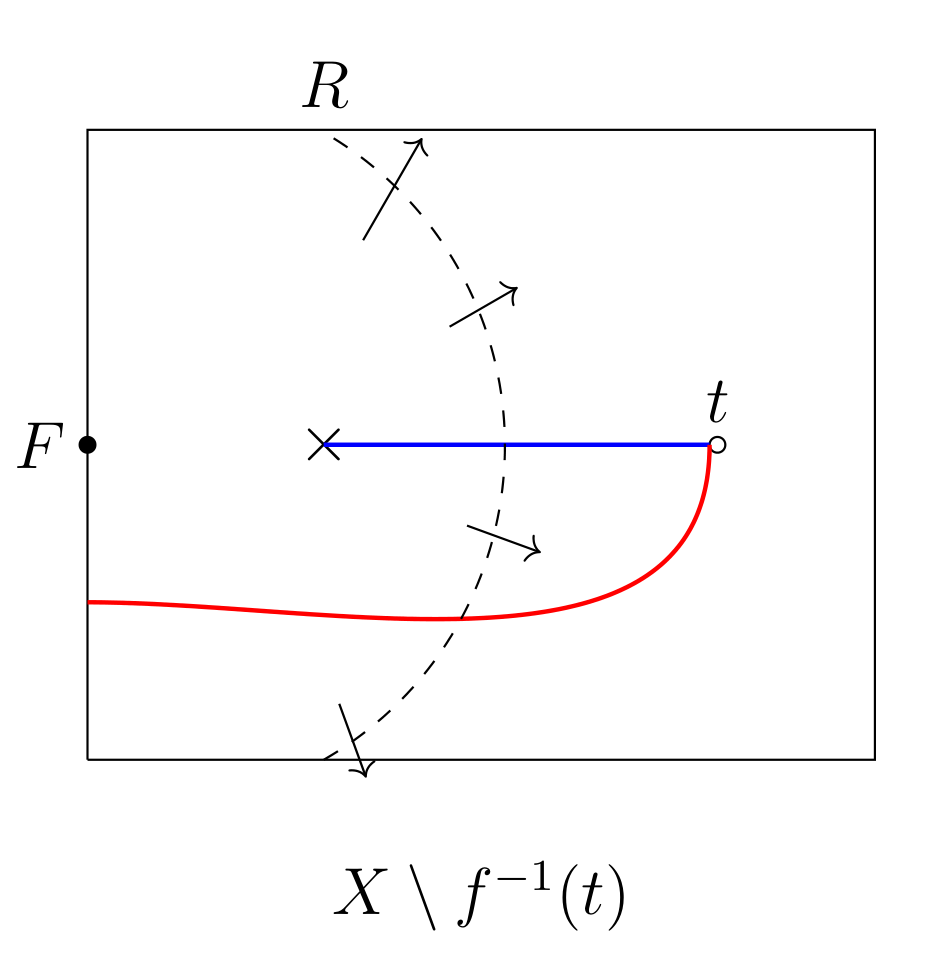
\includegraphics[width=0.36\textwidth]{figures/fig3_4.png}
  \caption{命题 \ref{prop:3-0-5} 中构造的子区域：对象 $L$ 为红色，余核 $\ell_i$ 为蓝色。}
  \label{fig:3-4}
\end{figure}

于是我们得到 $\cW(X,f)$ 的分裂生成元 $L$ 与 $\ell_i$（引理 \ref{lem:simple-homotopy}）。
但前者在该范畴中是平凡的，因为它们可经哈密顿推移到无穷远而与自身错开。
于是得到所要的分裂生成结论。
\end{proof}

\transnote{背景直觉：整个证明是「先在大空间里生成，再限制到子扇形，最后把多余生成元杀掉」。$L$ 在 $\cW(X,f)$ 中平凡，是因为它可被哈密顿推到无穷远，这一点正是「只有余核 $\ell_i$ 真正参与生成」的几何来源。}
